% Options for packages loaded elsewhere
% Options for packages loaded elsewhere
\PassOptionsToPackage{unicode}{hyperref}
\PassOptionsToPackage{hyphens}{url}
\PassOptionsToPackage{dvipsnames,svgnames,x11names}{xcolor}
%
\documentclass[
  spanish,
  11pt,
  a4paper,
  DIV=11,
  numbers=noendperiod]{scrartcl}
\usepackage{xcolor}
\usepackage[margin=2.5cm]{geometry}
\usepackage{amsmath,amssymb}
\setcounter{secnumdepth}{5}
\usepackage{iftex}
\ifPDFTeX
  \usepackage[T1]{fontenc}
  \usepackage[utf8]{inputenc}
  \usepackage{textcomp} % provide euro and other symbols
\else % if luatex or xetex
  \usepackage{unicode-math} % this also loads fontspec
  \defaultfontfeatures{Scale=MatchLowercase}
  \defaultfontfeatures[\rmfamily]{Ligatures=TeX,Scale=1}
\fi
\usepackage{lmodern}
\ifPDFTeX\else
  % xetex/luatex font selection
  \setmainfont[]{Times New Roman}
\fi
% Use upquote if available, for straight quotes in verbatim environments
\IfFileExists{upquote.sty}{\usepackage{upquote}}{}
\IfFileExists{microtype.sty}{% use microtype if available
  \usepackage[]{microtype}
  \UseMicrotypeSet[protrusion]{basicmath} % disable protrusion for tt fonts
}{}
\makeatletter
\@ifundefined{KOMAClassName}{% if non-KOMA class
  \IfFileExists{parskip.sty}{%
    \usepackage{parskip}
  }{% else
    \setlength{\parindent}{0pt}
    \setlength{\parskip}{6pt plus 2pt minus 1pt}}
}{% if KOMA class
  \KOMAoptions{parskip=half}}
\makeatother
% Make \paragraph and \subparagraph free-standing
\makeatletter
\ifx\paragraph\undefined\else
  \let\oldparagraph\paragraph
  \renewcommand{\paragraph}{
    \@ifstar
      \xxxParagraphStar
      \xxxParagraphNoStar
  }
  \newcommand{\xxxParagraphStar}[1]{\oldparagraph*{#1}\mbox{}}
  \newcommand{\xxxParagraphNoStar}[1]{\oldparagraph{#1}\mbox{}}
\fi
\ifx\subparagraph\undefined\else
  \let\oldsubparagraph\subparagraph
  \renewcommand{\subparagraph}{
    \@ifstar
      \xxxSubParagraphStar
      \xxxSubParagraphNoStar
  }
  \newcommand{\xxxSubParagraphStar}[1]{\oldsubparagraph*{#1}\mbox{}}
  \newcommand{\xxxSubParagraphNoStar}[1]{\oldsubparagraph{#1}\mbox{}}
\fi
\makeatother

\usepackage{color}
\usepackage{fancyvrb}
\newcommand{\VerbBar}{|}
\newcommand{\VERB}{\Verb[commandchars=\\\{\}]}
\DefineVerbatimEnvironment{Highlighting}{Verbatim}{commandchars=\\\{\}}
% Add ',fontsize=\small' for more characters per line
\usepackage{framed}
\definecolor{shadecolor}{RGB}{241,243,245}
\newenvironment{Shaded}{\begin{snugshade}}{\end{snugshade}}
\newcommand{\AlertTok}[1]{\textcolor[rgb]{0.68,0.00,0.00}{#1}}
\newcommand{\AnnotationTok}[1]{\textcolor[rgb]{0.37,0.37,0.37}{#1}}
\newcommand{\AttributeTok}[1]{\textcolor[rgb]{0.40,0.45,0.13}{#1}}
\newcommand{\BaseNTok}[1]{\textcolor[rgb]{0.68,0.00,0.00}{#1}}
\newcommand{\BuiltInTok}[1]{\textcolor[rgb]{0.00,0.23,0.31}{#1}}
\newcommand{\CharTok}[1]{\textcolor[rgb]{0.13,0.47,0.30}{#1}}
\newcommand{\CommentTok}[1]{\textcolor[rgb]{0.37,0.37,0.37}{#1}}
\newcommand{\CommentVarTok}[1]{\textcolor[rgb]{0.37,0.37,0.37}{\textit{#1}}}
\newcommand{\ConstantTok}[1]{\textcolor[rgb]{0.56,0.35,0.01}{#1}}
\newcommand{\ControlFlowTok}[1]{\textcolor[rgb]{0.00,0.23,0.31}{\textbf{#1}}}
\newcommand{\DataTypeTok}[1]{\textcolor[rgb]{0.68,0.00,0.00}{#1}}
\newcommand{\DecValTok}[1]{\textcolor[rgb]{0.68,0.00,0.00}{#1}}
\newcommand{\DocumentationTok}[1]{\textcolor[rgb]{0.37,0.37,0.37}{\textit{#1}}}
\newcommand{\ErrorTok}[1]{\textcolor[rgb]{0.68,0.00,0.00}{#1}}
\newcommand{\ExtensionTok}[1]{\textcolor[rgb]{0.00,0.23,0.31}{#1}}
\newcommand{\FloatTok}[1]{\textcolor[rgb]{0.68,0.00,0.00}{#1}}
\newcommand{\FunctionTok}[1]{\textcolor[rgb]{0.28,0.35,0.67}{#1}}
\newcommand{\ImportTok}[1]{\textcolor[rgb]{0.00,0.46,0.62}{#1}}
\newcommand{\InformationTok}[1]{\textcolor[rgb]{0.37,0.37,0.37}{#1}}
\newcommand{\KeywordTok}[1]{\textcolor[rgb]{0.00,0.23,0.31}{\textbf{#1}}}
\newcommand{\NormalTok}[1]{\textcolor[rgb]{0.00,0.23,0.31}{#1}}
\newcommand{\OperatorTok}[1]{\textcolor[rgb]{0.37,0.37,0.37}{#1}}
\newcommand{\OtherTok}[1]{\textcolor[rgb]{0.00,0.23,0.31}{#1}}
\newcommand{\PreprocessorTok}[1]{\textcolor[rgb]{0.68,0.00,0.00}{#1}}
\newcommand{\RegionMarkerTok}[1]{\textcolor[rgb]{0.00,0.23,0.31}{#1}}
\newcommand{\SpecialCharTok}[1]{\textcolor[rgb]{0.37,0.37,0.37}{#1}}
\newcommand{\SpecialStringTok}[1]{\textcolor[rgb]{0.13,0.47,0.30}{#1}}
\newcommand{\StringTok}[1]{\textcolor[rgb]{0.13,0.47,0.30}{#1}}
\newcommand{\VariableTok}[1]{\textcolor[rgb]{0.07,0.07,0.07}{#1}}
\newcommand{\VerbatimStringTok}[1]{\textcolor[rgb]{0.13,0.47,0.30}{#1}}
\newcommand{\WarningTok}[1]{\textcolor[rgb]{0.37,0.37,0.37}{\textit{#1}}}

\usepackage{longtable,booktabs,array}
\usepackage{calc} % for calculating minipage widths
% Correct order of tables after \paragraph or \subparagraph
\usepackage{etoolbox}
\makeatletter
\patchcmd\longtable{\par}{\if@noskipsec\mbox{}\fi\par}{}{}
\makeatother
% Allow footnotes in longtable head/foot
\IfFileExists{footnotehyper.sty}{\usepackage{footnotehyper}}{\usepackage{footnote}}
\makesavenoteenv{longtable}
\usepackage{graphicx}
\makeatletter
\newsavebox\pandoc@box
\newcommand*\pandocbounded[1]{% scales image to fit in text height/width
  \sbox\pandoc@box{#1}%
  \Gscale@div\@tempa{\textheight}{\dimexpr\ht\pandoc@box+\dp\pandoc@box\relax}%
  \Gscale@div\@tempb{\linewidth}{\wd\pandoc@box}%
  \ifdim\@tempb\p@<\@tempa\p@\let\@tempa\@tempb\fi% select the smaller of both
  \ifdim\@tempa\p@<\p@\scalebox{\@tempa}{\usebox\pandoc@box}%
  \else\usebox{\pandoc@box}%
  \fi%
}
% Set default figure placement to htbp
\def\fps@figure{htbp}
\makeatother



\ifLuaTeX
\usepackage[bidi=basic]{babel}
\else
\usepackage[bidi=default]{babel}
\fi
\ifPDFTeX
\else
\babelfont{rm}[]{Times New Roman}
\fi
% get rid of language-specific shorthands (see #6817):
\let\LanguageShortHands\languageshorthands
\def\languageshorthands#1{}


\setlength{\emergencystretch}{3em} % prevent overfull lines

\providecommand{\tightlist}{%
  \setlength{\itemsep}{0pt}\setlength{\parskip}{0pt}}



 


\usepackage{booktabs}
\usepackage{longtable}
\usepackage{array}
\usepackage{multirow}
\usepackage{wrapfig}
\usepackage{float}
\usepackage{colortbl}
\usepackage{pdflscape}
\usepackage{tabu}
\usepackage{threeparttable}
\usepackage{threeparttablex}
\usepackage[normalem]{ulem}
\usepackage{makecell}
\usepackage{xcolor}
\KOMAoption{captions}{tableheading}
\makeatletter
\@ifpackageloaded{caption}{}{\usepackage{caption}}
\AtBeginDocument{%
\ifdefined\contentsname
  \renewcommand*\contentsname{Tabla de contenidos}
\else
  \newcommand\contentsname{Tabla de contenidos}
\fi
\ifdefined\listfigurename
  \renewcommand*\listfigurename{Listado de Figuras}
\else
  \newcommand\listfigurename{Listado de Figuras}
\fi
\ifdefined\listtablename
  \renewcommand*\listtablename{Listado de Tablas}
\else
  \newcommand\listtablename{Listado de Tablas}
\fi
\ifdefined\figurename
  \renewcommand*\figurename{Figura}
\else
  \newcommand\figurename{Figura}
\fi
\ifdefined\tablename
  \renewcommand*\tablename{Tabla}
\else
  \newcommand\tablename{Tabla}
\fi
}
\@ifpackageloaded{float}{}{\usepackage{float}}
\floatstyle{ruled}
\@ifundefined{c@chapter}{\newfloat{codelisting}{h}{lop}}{\newfloat{codelisting}{h}{lop}[chapter]}
\floatname{codelisting}{Listado}
\newcommand*\listoflistings{\listof{codelisting}{Listado de Listados}}
\makeatother
\makeatletter
\makeatother
\makeatletter
\@ifpackageloaded{caption}{}{\usepackage{caption}}
\@ifpackageloaded{subcaption}{}{\usepackage{subcaption}}
\makeatother
\usepackage{bookmark}
\IfFileExists{xurl.sty}{\usepackage{xurl}}{} % add URL line breaks if available
\urlstyle{same}
\hypersetup{
  pdftitle={Análisis exploratorios},
  pdfauthor={Santos G},
  pdflang={es},
  colorlinks=true,
  linkcolor={blue},
  filecolor={Maroon},
  citecolor={Blue},
  urlcolor={Blue},
  pdfcreator={LaTeX via pandoc}}


\title{Análisis exploratorios}
\author{Santos G}
\date{}
\begin{document}
\maketitle

\renewcommand*\contentsname{Tabla de contenidos}
{
\hypersetup{linkcolor=}
\setcounter{tocdepth}{2}
\tableofcontents
}

\begin{Shaded}
\begin{Highlighting}[numbers=left,,]
\CommentTok{\# Librerías }
\FunctionTok{library}\NormalTok{(tidyverse)   }\CommentTok{\# Manipulación de datos: dplyr, tidyr, readr}
\FunctionTok{library}\NormalTok{(janitor)     }\CommentTok{\# Limpieza: clean\_names(), tabyl()}
\FunctionTok{library}\NormalTok{(ggplot2)     }\CommentTok{\# Gráficos profesionales}
\FunctionTok{library}\NormalTok{(skimr)       }\CommentTok{\# EDA rápido y completo (skim())}
\FunctionTok{library}\NormalTok{(GGally)      }\CommentTok{\# Matriz de gráficos para variables múltiples}
\FunctionTok{library}\NormalTok{(knitr)       }\CommentTok{\# Tablas en Quarto}
\FunctionTok{library}\NormalTok{(kableExtra)  }\CommentTok{\# Tablas formateadas para informes}
\end{Highlighting}
\end{Shaded}

\section{Contexto del proyecto}\label{contexto-del-proyecto}

Se realizó una exploración y control de calidad de los datos de entrada
para identificar variables relevantes, evaluar supuestos básicos y
priorizar rutas analíticas. El objetivo es generar una guía reproducible
que permita a futuros analistas (o a un equipo de consultoría) replicar
y ampliar los análisis según objetivos específicos (p.~ej. comparar
tratamientos, modelar abundancias o construir índices de condición).

\section{Carga y verificación inicial de
datos}\label{carga-y-verificaciuxf3n-inicial-de-datos}

El dataset contiene \textbf{N = 150 observaciones} y \textbf{5
variables}. Cuatro son cuantitativas continuas en centímetros
(\emph{Sepal.Length, Sepal.Width, Petal.Length, Petal.Width}), y una
categórica (\emph{Species}), que clasifica en tres grupos balanceados (n
= 50 por especie). No se detectaron valores faltantes ni duplicados tras
la inspección inicial. Esta estructura balanceada y sin NA permite
aplicar análisis univariados, comparativos y multivariados con mínimo
preprocesamiento.

La \textbf{Tabla 1} de estadísticos descriptivos muestra lo siguiente:

\begin{itemize}
\item
  \textbf{Sepal.Length:} media ≈ 5.84 cm, SD ≈ 0.83, rango 4.3--7.9.
  Variación moderada, con solapamiento esperado entre especies.
\item
  \textbf{Sepal.Width:} media ≈ 3.06 cm, SD ≈ 0.44, rango 2.0--4.4. Es
  la variable más estable, aunque con ligera asimetría negativa.
\item
  \textbf{Petal.Length:} media ≈ 3.76 cm, SD ≈ 1.77, rango 1.0--6.9.
  Mayor dispersión relativa, con clara separación de \emph{setosa}.
\item
  \textbf{Petal.Width:} media ≈ 1.20 cm, SD ≈ 0.76, rango 0.1--2.5. Alta
  variabilidad, con potencial de discriminación entre las tres especies.
\end{itemize}

\begin{Shaded}
\begin{Highlighting}[numbers=left,,]
\CommentTok{\#|label: data{-}load}

\CommentTok{\# Carga de datos (ejemplo iris) y limpieza mínima}
\FunctionTok{data}\NormalTok{(}\StringTok{"iris"}\NormalTok{)}
\NormalTok{df }\OtherTok{\textless{}{-}} \FunctionTok{as\_tibble}\NormalTok{(iris) }\SpecialCharTok{\%\textgreater{}\%} 
\NormalTok{  janitor}\SpecialCharTok{::}\FunctionTok{clean\_names}\NormalTok{()   }\CommentTok{\# convierte a snake\_case: sepal\_length, etc.}

\CommentTok{\# Información básica}
\NormalTok{n\_rows }\OtherTok{\textless{}{-}} \FunctionTok{nrow}\NormalTok{(df); n\_cols }\OtherTok{\textless{}{-}} \FunctionTok{ncol}\NormalTok{(df)}
\NormalTok{tbl1}\OtherTok{\textless{}{-}}\FunctionTok{skim}\NormalTok{(df) }
\NormalTok{tbl1 }\CommentTok{\# Resumen compacto por variable}
\end{Highlighting}
\end{Shaded}

\begin{longtable}[]{@{}ll@{}}
\caption{Data summary}\tabularnewline
\toprule\noalign{}
\endfirsthead
\endhead
\bottomrule\noalign{}
\endlastfoot
Name & df \\
Number of rows & 150 \\
Number of columns & 5 \\
\_\_\_\_\_\_\_\_\_\_\_\_\_\_\_\_\_\_\_\_\_\_\_ & \\
Column type frequency: & \\
factor & 1 \\
numeric & 4 \\
\_\_\_\_\_\_\_\_\_\_\_\_\_\_\_\_\_\_\_\_\_\_\_\_ & \\
Group variables & None \\
\end{longtable}

\textbf{Variable type: factor}

\begin{longtable}[]{@{}
  >{\raggedright\arraybackslash}p{(\linewidth - 10\tabcolsep) * \real{0.1728}}
  >{\raggedleft\arraybackslash}p{(\linewidth - 10\tabcolsep) * \real{0.1235}}
  >{\raggedleft\arraybackslash}p{(\linewidth - 10\tabcolsep) * \real{0.1728}}
  >{\raggedright\arraybackslash}p{(\linewidth - 10\tabcolsep) * \real{0.0988}}
  >{\raggedleft\arraybackslash}p{(\linewidth - 10\tabcolsep) * \real{0.1111}}
  >{\raggedright\arraybackslash}p{(\linewidth - 10\tabcolsep) * \real{0.3210}}@{}}
\toprule\noalign{}
\begin{minipage}[b]{\linewidth}\raggedright
skim\_variable
\end{minipage} & \begin{minipage}[b]{\linewidth}\raggedleft
n\_missing
\end{minipage} & \begin{minipage}[b]{\linewidth}\raggedleft
complete\_rate
\end{minipage} & \begin{minipage}[b]{\linewidth}\raggedright
ordered
\end{minipage} & \begin{minipage}[b]{\linewidth}\raggedleft
n\_unique
\end{minipage} & \begin{minipage}[b]{\linewidth}\raggedright
top\_counts
\end{minipage} \\
\midrule\noalign{}
\endhead
\bottomrule\noalign{}
\endlastfoot
species & 0 & 1 & FALSE & 3 & set: 50, ver: 50, vir: 50 \\
\end{longtable}

\textbf{Variable type: numeric}

\begin{longtable}[]{@{}
  >{\raggedright\arraybackslash}p{(\linewidth - 20\tabcolsep) * \real{0.1842}}
  >{\raggedleft\arraybackslash}p{(\linewidth - 20\tabcolsep) * \real{0.1316}}
  >{\raggedleft\arraybackslash}p{(\linewidth - 20\tabcolsep) * \real{0.1842}}
  >{\raggedleft\arraybackslash}p{(\linewidth - 20\tabcolsep) * \real{0.0658}}
  >{\raggedleft\arraybackslash}p{(\linewidth - 20\tabcolsep) * \real{0.0658}}
  >{\raggedleft\arraybackslash}p{(\linewidth - 20\tabcolsep) * \real{0.0526}}
  >{\raggedleft\arraybackslash}p{(\linewidth - 20\tabcolsep) * \real{0.0526}}
  >{\raggedleft\arraybackslash}p{(\linewidth - 20\tabcolsep) * \real{0.0658}}
  >{\raggedleft\arraybackslash}p{(\linewidth - 20\tabcolsep) * \real{0.0526}}
  >{\raggedleft\arraybackslash}p{(\linewidth - 20\tabcolsep) * \real{0.0658}}
  >{\raggedright\arraybackslash}p{(\linewidth - 20\tabcolsep) * \real{0.0789}}@{}}
\toprule\noalign{}
\begin{minipage}[b]{\linewidth}\raggedright
skim\_variable
\end{minipage} & \begin{minipage}[b]{\linewidth}\raggedleft
n\_missing
\end{minipage} & \begin{minipage}[b]{\linewidth}\raggedleft
complete\_rate
\end{minipage} & \begin{minipage}[b]{\linewidth}\raggedleft
mean
\end{minipage} & \begin{minipage}[b]{\linewidth}\raggedleft
sd
\end{minipage} & \begin{minipage}[b]{\linewidth}\raggedleft
p0
\end{minipage} & \begin{minipage}[b]{\linewidth}\raggedleft
p25
\end{minipage} & \begin{minipage}[b]{\linewidth}\raggedleft
p50
\end{minipage} & \begin{minipage}[b]{\linewidth}\raggedleft
p75
\end{minipage} & \begin{minipage}[b]{\linewidth}\raggedleft
p100
\end{minipage} & \begin{minipage}[b]{\linewidth}\raggedright
hist
\end{minipage} \\
\midrule\noalign{}
\endhead
\bottomrule\noalign{}
\endlastfoot
sepal\_length & 0 & 1 & 5.84 & 0.83 & 4.3 & 5.1 & 5.80 & 6.4 & 7.9 &
▆▇▇▅▂ \\
sepal\_width & 0 & 1 & 3.06 & 0.44 & 2.0 & 2.8 & 3.00 & 3.3 & 4.4 &
▁▆▇▂▁ \\
petal\_length & 0 & 1 & 3.76 & 1.77 & 1.0 & 1.6 & 4.35 & 5.1 & 6.9 &
▇▁▆▇▂ \\
petal\_width & 0 & 1 & 1.20 & 0.76 & 0.1 & 0.3 & 1.30 & 1.8 & 2.5 &
▇▁▇▅▃ \\
\end{longtable}

Aspectos destacados del dataset:

\begin{itemize}
\item
  \textbf{Escala homogénea de medidas:} todas las variables en
  centímetros → comparaciones y análisis multivariados sin necesidad de
  reescalado inmediato.
\item
  \textbf{Colinealidad esperada:} Petal.Length y Petal.Width muestran
  alta correlación, lo que debe considerarse en regresiones o PCA.
\item
  \textbf{Grupos biológicos claros y balanceados:} un escenario ideal
  para aprendizaje, aunque poco frecuente en estudios ecológicos reales.
\item
  \textbf{Potencial de discriminación:} las variables de pétalos
  concentran el mayor poder de separación, coherente con su relevancia
  funcional en la biología reproductiva de las plantas.
\end{itemize}

\section{Matriz de correlaciones y distribuciones entre variables
numéricas}\label{matriz-de-correlaciones-y-distribuciones-entre-variables-numuxe9ricas}

La \textbf{Figura 1} combina tres tipos de información: distribuciones
univariadas, relaciones bivariadas y correlacciones númericas.

\begin{Shaded}
\begin{Highlighting}[numbers=left,,]
\NormalTok{num\_df }\OtherTok{\textless{}{-}}\NormalTok{ df }\SpecialCharTok{\%\textgreater{}\%} \FunctionTok{select}\NormalTok{(}\FunctionTok{where}\NormalTok{(is.numeric))}
\NormalTok{Fig1}\OtherTok{\textless{}{-}}\NormalTok{ GGally}\SpecialCharTok{::}\FunctionTok{ggpairs}\NormalTok{(}
\NormalTok{  df,}
  \AttributeTok{columns =} \DecValTok{1}\SpecialCharTok{:}\DecValTok{4}\NormalTok{, }\CommentTok{\# solo variables numéricas}
  \AttributeTok{mapping =} \FunctionTok{aes}\NormalTok{(}\AttributeTok{color =}\NormalTok{ species), }\CommentTok{\# color por especie}
  \AttributeTok{upper =} \FunctionTok{list}\NormalTok{(}\AttributeTok{continuous =} \FunctionTok{wrap}\NormalTok{(}\StringTok{"cor"}\NormalTok{, }\AttributeTok{size =} \DecValTok{3}\NormalTok{)),}
  \AttributeTok{diag =} \FunctionTok{list}\NormalTok{(}\AttributeTok{continuous =} \FunctionTok{wrap}\NormalTok{(}\StringTok{"densityDiag"}\NormalTok{, }\AttributeTok{alpha =} \FloatTok{0.6}\NormalTok{))}
\NormalTok{)}
\NormalTok{Fig1}
\end{Highlighting}
\end{Shaded}

\begin{figure}[H]

{\centering \pandocbounded{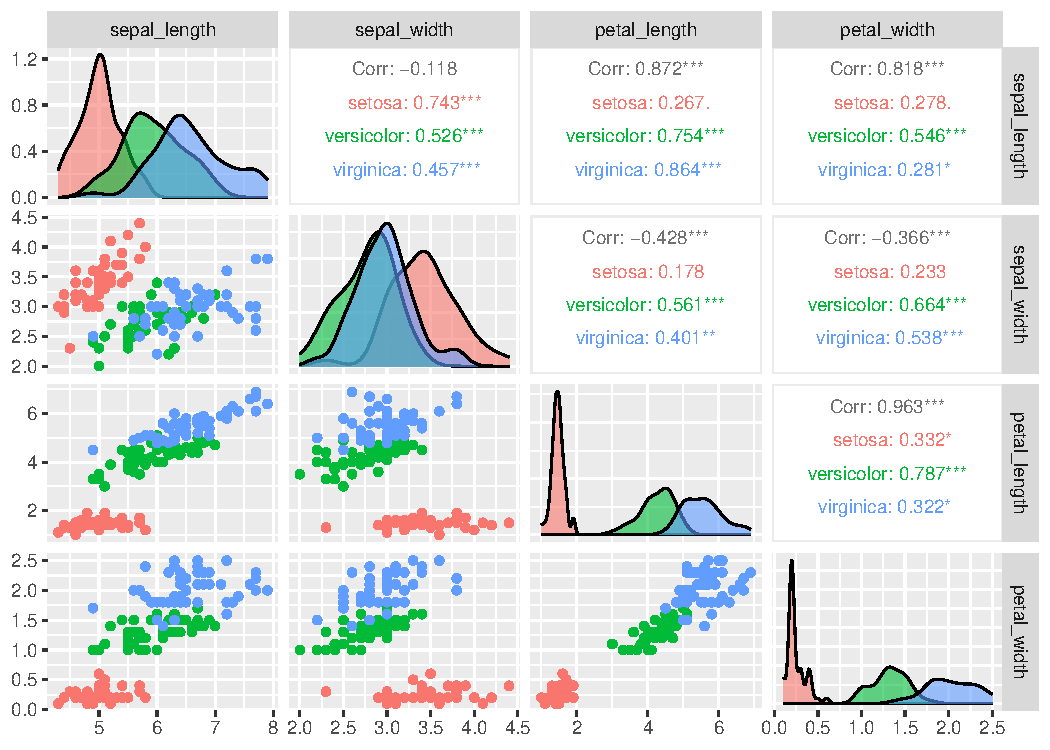
\includegraphics[keepaspectratio]{Análisis-exploratorio_files/figure-pdf/ggpairs-1.pdf}}

}

\caption{Matriz de dispersión y correlación de las variables
cuantitativas.}

\end{figure}%

\subsection{Distribuciones
univariadas}\label{distribuciones-univariadas}

\begin{itemize}
\tightlist
\item
  \textbf{Sepal.Length}:

  \begin{itemize}
  \tightlist
  \item
    \emph{Setosa}: concentrada en valores bajos (4.3 - 5.8 cm), muy
    homogénea.\\
  \item
    \emph{Versicolor}: rango intermedio (≈ 4.9 - 7.0 cm).\\
  \item
    \emph{Virginica}: valores altos (≈ 4.9 - 7.9 cm), con ligera
    superposición con Versicolor.\\
  \item
    \textbf{Interpretación}: útil para separar \emph{Setosa}, pero
    \emph{Versicolor} y \emph{Virginica} se solapan.
  \end{itemize}
\item
  \textbf{Sepal.Width}:

  \begin{itemize}
  \tightlist
  \item
    Distribución amplia en todas las especies.\\
  \item
    \emph{Setosa} tiende a mayores valores promedio, pero con
    solapamiento considerable.\\
  \item
    \textbf{Interpretación}: poco poder discriminante, refleja
    variabilidad natural en la anchura del sépalo.
  \end{itemize}
\item
  \textbf{Petal.Length}:

  \begin{itemize}
  \tightlist
  \item
    \emph{Setosa}: valores muy bajos (≈ 1.0 - 1.9 cm), sin solapamiento
    con las otras especies.\\
  \item
    \emph{Versicolor}: rango medio (≈ 3.0 - 5.1 cm).\\
  \item
    \emph{Virginica}: valores altos (≈ 4.5 - 6.9 cm).\\
  \item
    \textbf{Interpretación}: variable clave, separa \emph{Setosa} y
    discrimina bastante bien \emph{Versicolor} vs \emph{Virginica}.
  \end{itemize}
\item
  \textbf{Petal.Width}:

  \begin{itemize}
  \tightlist
  \item
    \emph{Setosa}: valores muy bajos (≈ 0.1 - 0.6 cm).\\
  \item
    \emph{Versicolor}: rango medio (≈ 1.0 - 1.8 cm).\\
  \item
    \emph{Virginica}: valores altos (≈ 1.4 - 2.5 cm).\\
  \item
    \textbf{Interpretación}: la más robusta para separar las tres
    especies, casi sin solapamiento.
  \end{itemize}
\end{itemize}

\subsection{Relaciones bivariadas}\label{relaciones-bivariadas}

\begin{itemize}
\tightlist
\item
  \textbf{Sepal.Length vs Sepal.Width}: gran solapamiento entre
  especies, con nubes de puntos mezcladas. \emph{Setosa} muestra ligera
  tendencia a sépalos más anchos.

  \begin{itemize}
  \tightlist
  \item
    \textbf{Interpretación}: baja capacidad de discriminación.
  \end{itemize}
\item
  \textbf{Sepal.Length vs Petal.Length}: patrón positivo moderado.
  \emph{Setosa} queda claramente apartada (pétalos muy cortos).
  \emph{Versicolor} y \emph{Virginica} siguen una línea ascendente, con
  solapamiento parcial.

  \begin{itemize}
  \tightlist
  \item
    \textbf{Interpretación}: ayuda a diferenciar \emph{Setosa}, pero no
    tanto entre las otras dos.
  \end{itemize}
\item
  \textbf{Sepal.Length vs Petal.Width}: tendencia positiva clara.
  \emph{Setosa} aislada (pétalos estrechos). \emph{Virginica} tiende a
  valores más altos.

  \begin{itemize}
  \tightlist
  \item
    \textbf{Interpretación}: más útil que \emph{Sepal.Length} solo, pero
    aún con solapamientos.
  \end{itemize}
\item
  \textbf{Sepal.Width vs Petal.Length}: relación débil, nubes muy
  mezcladas. \emph{Setosa} separada por bajos valores de pétalo, no por
  el sépalo.

  \begin{itemize}
  \tightlist
  \item
    \textbf{Interpretación}: variable \emph{Sepal.Width} poco
    informativa.
  \end{itemize}
\item
  \textbf{Sepal.Width vs Petal.Width}: relación débil, con gran
  dispersión. \emph{Setosa} se distingue porque tiene pétalos angostos,
  no por anchura del sépalo.

  \begin{itemize}
  \tightlist
  \item
    \textbf{Interpretación}: no aporta discriminación extra.
  \end{itemize}
\item
  \textbf{Petal.Length vs Petal.Width}: relación lineal muy fuerte, tres
  grupos claramente separados. \emph{Setosa} aislada en valores bajos;
  \emph{Versicolor} intermedia; \emph{Virginica} en el rango alto.

  \begin{itemize}
  \tightlist
  \item
    \textbf{Interpretación}: la combinación de estas dos variables es la
    mejor para clasificar especies.
  \end{itemize}
\end{itemize}

\subsection{Correlaciones numéricas}\label{correlaciones-numuxe9ricas}

\begin{itemize}
\tightlist
\item
  \textbf{Petal.Length vs Petal.Width}: r ≈ 0.96 (correlación muy alta).
  Variables casi redundantes, pero en conjunto definen un espacio
  morfológico clave.\\
\item
  \textbf{Sepal.Length vs Petal.Length}: r ≈ 0.87 (correlación fuerte).
  A mayor sépalo, mayor pétalo, patrón general de tamaño.\\
\item
  \textbf{Sepal.Length vs Petal.Width}: r ≈ 0.82 (correlación alta).
  También refleja el gradiente de tamaño floral.\\
\item
  \textbf{Sepal.Width con el resto}: correlaciones bajas (r entre -0.4 y
  0.3). Confirma que aporta poca información discriminante.
\end{itemize}

\subsection{Interpretación ecológica
general}\label{interpretaciuxf3n-ecoluxf3gica-general}

\begin{itemize}
\tightlist
\item
  Los \textbf{pétalos} son rasgos reproductivos clave: su longitud y
  anchura diferencian a las especies porque están ligados a estrategias
  de atracción de polinizadores.\\
\item
  Los \textbf{sépalos}, en cambio, son más plásticos y menos
  específicos, lo que explica su bajo poder discriminante.\\
\item
  La \textbf{correlación entre variables de pétalo} refleja que ambas
  describen el mismo fenómeno biológico (tamaño floral), pero su
  combinación refuerza la clasificación.\\
\item
  En un contexto real de ecología vegetal, esto sugiere que la
  diferenciación entre especies del género \emph{Iris} depende más de
  rasgos reproductivos (pétalos) que de rasgos de soporte (sépalos).
\end{itemize}

\section{Distribución de variables morfométricas entre
especies}\label{distribuciuxf3n-de-variables-morfomuxe9tricas-entre-especies}

La \textbf{Figura 2} presenta diagramas de caja y bigotes que resumen la
variación de las cuatro variables morfométricas en las tres especies de
\emph{Iris}. Este análisis complementa al resumen numérico y a la matriz
de relaciones bivariadas, ya que enfatiza tendencias centrales,
dispersión y presencia de datos atípicos.

\begin{Shaded}
\begin{Highlighting}[numbers=left,,]
\CommentTok{\# Pasar el dataset a formato largo}
\NormalTok{iris\_long }\OtherTok{\textless{}{-}}\NormalTok{ df }\SpecialCharTok{\%\textgreater{}\%}
  \FunctionTok{pivot\_longer}\NormalTok{(}\AttributeTok{cols =} \SpecialCharTok{{-}}\NormalTok{species,}
               \AttributeTok{names\_to =} \StringTok{"Variable"}\NormalTok{,}
               \AttributeTok{values\_to =} \StringTok{"Valor"}\NormalTok{)}

\CommentTok{\# Gráfico unificado}
\NormalTok{Fig2 }\OtherTok{\textless{}{-}} \FunctionTok{ggplot}\NormalTok{(iris\_long, }\FunctionTok{aes}\NormalTok{(}\AttributeTok{x =}\NormalTok{ species, }\AttributeTok{y =}\NormalTok{ Valor, }\AttributeTok{fill =}\NormalTok{ species)) }\SpecialCharTok{+}
  \FunctionTok{geom\_boxplot}\NormalTok{(}\AttributeTok{outlier.shape =} \DecValTok{21}\NormalTok{, }\AttributeTok{alpha =} \FloatTok{0.7}\NormalTok{) }\SpecialCharTok{+}
  \FunctionTok{facet\_wrap}\NormalTok{(}\SpecialCharTok{\textasciitilde{}}\NormalTok{ Variable, }\AttributeTok{scales =} \StringTok{"free\_y"}\NormalTok{) }\SpecialCharTok{+}
  \FunctionTok{labs}\NormalTok{(}
    \AttributeTok{title =} \StringTok{"Comparación de variables morfométricas en especies de Iris"}\NormalTok{,}
    \AttributeTok{x =} \StringTok{"Especies"}\NormalTok{,}
    \AttributeTok{y =} \StringTok{"Valor (cm)"}
\NormalTok{  ) }\SpecialCharTok{+}
  \FunctionTok{theme\_minimal}\NormalTok{(}\AttributeTok{base\_size =} \DecValTok{13}\NormalTok{) }\SpecialCharTok{+}
  \FunctionTok{theme}\NormalTok{(}
    \AttributeTok{plot.title =} \FunctionTok{element\_text}\NormalTok{(}\AttributeTok{hjust =} \FloatTok{0.5}\NormalTok{, }\AttributeTok{face =} \StringTok{"bold"}\NormalTok{),}
    \AttributeTok{legend.position =} \StringTok{"none"}\NormalTok{,}
    \AttributeTok{strip.text =} \FunctionTok{element\_text}\NormalTok{(}\AttributeTok{face =} \StringTok{"bold"}\NormalTok{)}
\NormalTok{  )}
\NormalTok{Fig2}
\end{Highlighting}
\end{Shaded}

\begin{figure}[H]

{\centering \pandocbounded{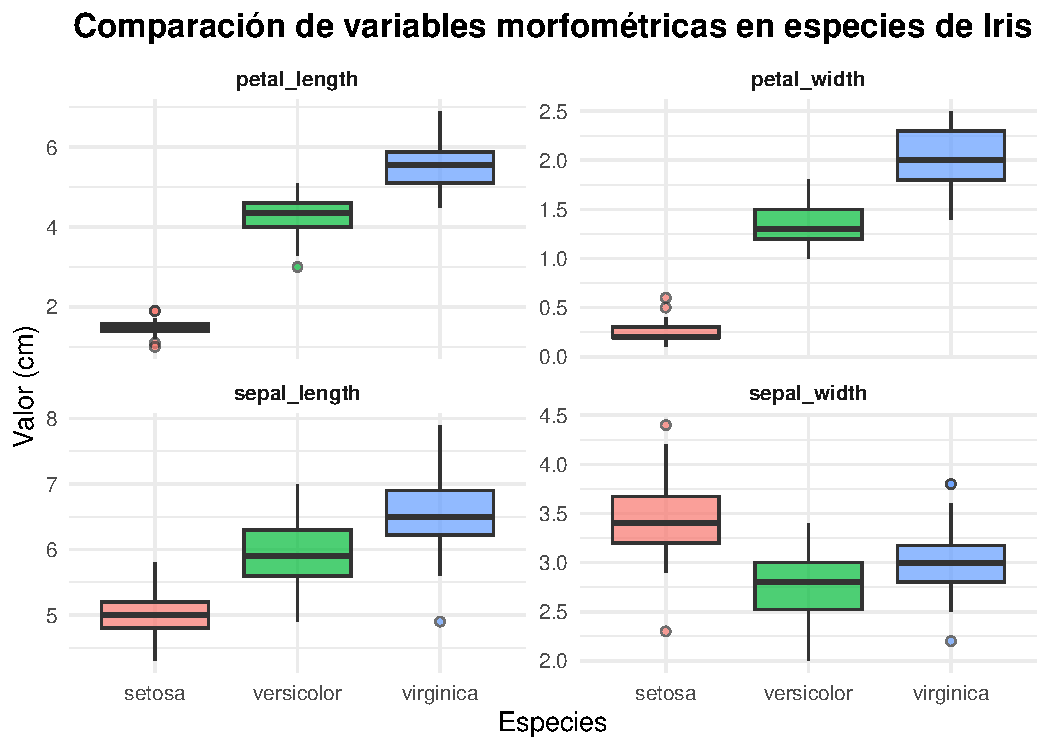
\includegraphics[keepaspectratio]{Análisis-exploratorio_files/figure-pdf/caja y bigotes-1.pdf}}

}

\caption{Distribución de variables morfométricas en tres especies de
Iris.}

\end{figure}%

\subsection{Sepal.Length (longitud del
sépalo)}\label{sepal.length-longitud-del-suxe9palo}

\begin{itemize}
\tightlist
\item
  \emph{I. setosa} muestra valores concentrados entre \textbf{4.3 y 5.8
  cm}, con una mediana cercana a \textbf{5.0 cm}. La caja es compacta,
  indicando baja variabilidad.\\
\item
  \emph{I. versicolor} se distribuye entre \textbf{4.9 y 7.0 cm}, con
  mediana ≈ \textbf{5.9 cm}, rango intermedio.\\
\item
  \emph{I. virginica} alcanza los valores más altos (\textbf{4.9--7.9
  cm}), con mediana ≈ \textbf{6.5 cm}.
\end{itemize}

\textbf{Interpretación}: hay cierto solapamiento entre \emph{versicolor}
y \emph{virginica}. Útil para distinguir a \emph{setosa}, pero no para
discriminar con precisión entre \emph{versicolor} y \emph{virginica}.

\subsection{Sepal.Width (anchura del
sépalo)}\label{sepal.width-anchura-del-suxe9palo}

\begin{itemize}
\item
  \emph{I. setosa} tiene la mediana más alta (≈ \textbf{3.4 cm}), con
  valores entre \textbf{2.3 y 4.4 cm}.\\
\item
  \emph{I. versicolor} oscila entre \textbf{2.0 y 3.4 cm}, mediana ≈
  \textbf{2.8 cm}.\\
\item
  \emph{I. virginica} se ubica entre \textbf{2.2 y 3.8 cm}, mediana ≈
  \textbf{3.0 cm}.
\item
  Se observan varios outliers tanto en \emph{setosa} como
  \emph{virginica,} individuos con sépalos inusualmente estrechos. Estos
  valores atípicos podrían reflejar variación intraespecífica natural o
  condiciones ambientales particulares. La fuerte dispersión y el
  solapamiento reducen el valor discriminante de esta variable.
\end{itemize}

\textbf{Interpretación}: aunque setosa tiende a mayor anchura, la amplia
dispersión y solapamiento hacen que esta variable tenga bajo poder
discriminante.

\subsection{Petal.Length (longitud del
pétalo)}\label{petal.length-longitud-del-puxe9talo}

\begin{itemize}
\tightlist
\item
  \emph{I. setosa} presenta valores muy bajos (\textbf{1.0--1.9 cm}) con
  mediana ≈ \textbf{1.5 cm}.\\
\item
  \emph{I. versicolor} ocupa un rango intermedio (\textbf{3.0--5.1 cm}),
  con mediana ≈ \textbf{4.3 cm}.\\
\item
  \emph{I. virginica} concentra los valores más altos (\textbf{4.5--6.9
  cm}), mediana ≈ \textbf{5.5 cm}.
\end{itemize}

\textbf{Interpretación}: el solapamiento entre \emph{versicolor} y
\emph{virginica} es reducido y se da en los límites
superiores/inferiores de sus cajas. Esta variable es altamente
informativa; separa completamente a \emph{setosa} y discrimina en gran
medida a \emph{versicolor} y \emph{virginica}.

\subsection{Petal.Width (anchura del
pétalo)}\label{petal.width-anchura-del-puxe9talo}

\begin{itemize}
\tightlist
\item
  \emph{I. setosa} tiene los valores más bajos (\textbf{0.1--0.6 cm}),
  con mediana ≈ \textbf{0.2 cm}, sin solapamiento con las otras
  especies.\\
\item
  \emph{I. versicolor} se concentra entre \textbf{1.0 y 1.8 cm}, mediana
  ≈ \textbf{1.3 cm}.\\
\item
  \emph{I. virginica} presenta los valores más altos (\textbf{1.4--2.5
  cm}), mediana ≈ \textbf{2.0 cm}.
\end{itemize}

\textbf{Interpretación}: junto con \emph{Petal.Length}, constituye la
variable más robusta para separar especies; su poder discriminante es
muy alto y con solapamiento mínimo.

\subsection{Interpretación general}\label{interpretaciuxf3n-general}

Las variables de pétalo muestran diferencias netas entre especies, con
cajas bien separadas. Por lo que se considera un rasgo clave para
clasificación, debido a su alta capacidad de separar grupos. A
diferencias de las variables de sépalo que presentan mayor dispersión y
solapamiento, lo que limita su valor clasificatorio, debido a su menor
capacidad diagnóstica, más influenciados por plasticidad ambiental.

El patrón confirma que los caracteres reproductivos (pétalos) son más
determinantes para la diferenciación interespecífica, mientras que los
vegetativos (sépalos) presentan mayor variabilidad y menor poder
diagnóstico.




\end{document}
